% Stochastic conditional FM pilot: a four-slide appendix (FLOW_NOTES.md,
% "Stochastic conditional FM pilot"). Numbers: docs/flow/translation/condfm/*.csv
% (translation_report.py, condfm_report.py) via tables/cf_*.tex; figures
% ../cf_*.png and ../deck/*.png. Build:
%   cd docs/flow/translation/condfm/slides && ~/pyext/tectonic_env/bin/tectonic condfm_appendix.tex
\documentclass[aspectratio=169,10pt]{beamer}
\usetheme{default}
\setbeamertemplate{navigation symbols}{}

\usepackage{booktabs}
\usepackage{graphicx}
\usepackage{xcolor}
\usepackage{amsmath}
\graphicspath{{../}{../deck/}}

% ink and series colours of the figures (blue / aqua / yellow / violet pass the
% colour-vision check; the arms also differ in line style)
\definecolor{ink}{HTML}{0B0B0B}
\definecolor{ink2}{HTML}{52514E}
\definecolor{muted}{HTML}{898781}
\definecolor{rule}{HTML}{E1E0D9}
\definecolor{wash}{HTML}{F4F3EF}
\definecolor{cOT}{HTML}{2A78D6}
\definecolor{cHD}{HTML}{1BAF7A}
\definecolor{cSF}{HTML}{EDA100}
\definecolor{cRJ}{HTML}{4A3AA7}

\setbeamercolor{normal text}{fg=ink}
\setbeamercolor{frametitle}{fg=ink}
\setbeamercolor{itemize item}{fg=muted}
\setbeamercolor{itemize subitem}{fg=muted}
\setbeamerfont{frametitle}{size=\large,series=\bfseries}
\setbeamertemplate{itemize items}{\raisebox{0.15em}{\scalebox{0.6}{$\blacksquare$}}}
\setbeamertemplate{itemize subitem}{--}
\setbeamersize{text margin left=1.1em,text margin right=1.1em}
\setbeamertemplate{frametitle}{\vspace{0.45em}\insertframetitle\par\vspace{-0.25em}%
  {\color{rule}\rule{\textwidth}{0.6pt}}}
\setbeamertemplate{footline}{\hspace{1.1em}{\tiny\color{muted}Appendix: stochastic conditional
  flow matching, PYTHIA $\to$ JEWEL, seed 0, 2026-10-05}\hfill{\tiny\color{muted}S\insertframenumber}%
  \hspace{1.1em}\vspace{0.6em}}

% line keys in the series colours, then the name in ink
\newcommand{\keyot}{{\color{cOT}\rule[0.25em]{1.1em}{1.6pt}}\,}
\newcommand{\keyhd}{{\color{cHD}\rule[0.25em]{0.45em}{1.6pt}\hspace{0.2em}\rule[0.25em]{0.45em}{1.6pt}}\,}
\newcommand{\keysf}{{\color{cSF}\rule[0.25em]{0.6em}{1.6pt}\hspace{0.15em}\rule[0.25em]{0.15em}{1.6pt}}\,}
\newcommand{\keyrj}{{\color{cRJ}\rule[0.25em]{0.6em}{1.6pt}\hspace{0.15em}\rule[0.25em]{0.15em}{1.6pt}}\,}
\newcommand{\ot}{\textbf{OT-FM}}
\newcommand{\hda}{\textbf{hard}}
\newcommand{\sfa}{\textbf{soft}}
\newcommand{\snote}[1]{{\scriptsize\color{ink2}#1\par}}
\newcommand{\refs}[1]{{\scriptsize\color{muted}[#1]}}

\begin{document}

% ---------------------------------------------------------------- S1
\begin{frame}{S1. Setup: several JEWEL-like jets per PYTHIA jet}
\begin{columns}[T]
\column{0.5\textwidth}
\scriptsize
\textbf{Question.} \ot{} (the deterministic OT-CFM translator) gives one output per PYTHIA jet. Can
noise-driven conditional flow matching keep its JEWEL-like populations and input dependence, with sharp,
different samples of each jet? Exploratory: the conditional distribution is the one the pairing
defines, not a physical medium response.

\vspace{0.3em}
\textbf{Model} (standard flow matching \refs{Lipman et al., arXiv:2210.02747}; not DSBM, not an SDE
bridge)
\begin{itemize}\setlength\itemsep{0.1em}
\item $x_t = (1-t)\,\epsilon + t\,y$, \ $u_t = y - \epsilon$, \
  $\mathcal{L} = \big\langle (v_\theta(t, [x_t, c]) - u_t)^2 \big\rangle$; $c$: the PYTHIA jet, an
  unchanged second input channel; $y$: its paired JEWEL training jet; $\epsilon$: Gaussian on the 53
  cone towers
\item sampling: fix $c$, draw $\epsilon$, midpoint ODE with 128 calls; the same $(c, \epsilon)$ give
  the same jet
\item \textbf{pairs} \refs{Tong et al., arXiv:2302.00482}: in each batch of 256 PYTHIA and 256 JEWEL
  training jets a plan on the squared $L^2$ of the standardised $\log(E + 0.1)$ canvases, one target
  drawn per condition. \keyhd\hda{}: exact OT. \keysf\sfa{}: entropic OT, reg 7, i.e.\ a median of 4
  targets per row (5-95\%: 1.6-9.2), fixed on training jets before training
\item equal in both: data, batches, times, noise, initialisation, the UVCGAN-S network (2 input
  channels), seed 0, 2 A6000 GPU-hours
\end{itemize}
\column{0.48\textwidth}
\scriptsize
\textbf{The training pairs themselves} (8192 pairs, before training)

\vspace{0.2em}
\scriptsize
\setlength{\tabcolsep}{2pt}
\begin{tabular}{lrrrr}
\toprule
 & EMD & $r(p_T)$ & $r$(girth) & rms $\Delta p_T$ \\
\midrule
\keyhd exact plan (hard) & 0.235 & 0.17 & 0.71 & 11.8 \\
\keysf entropic plan (soft) & 0.240 & 0.16 & 0.70 & 11.9 \\
random pairs & 0.465 & 0.00 & 0.02 & 12.7 \\
\midrule
\keyot OT-FM output vs its input & 0.041 & 0.94 & 0.99 & 6.6 \\
\bottomrule
\end{tabular}


\vspace{0.2em}
\snote{$r$: correlation of a condition's and its target's observable. An OT partner shares part of the
condition's width and almost none of its $p_T$.}

\vspace{0.5em}
\textbf{Checks}
\begin{itemize}\setlength\itemsep{0.1em}
\item path in the loss, pair indices, fixed-noise repeats: exact
\item Gaussian control $y = c + 0.2\,\xi$: samples of a fixed $c$ have mean within 0.013 of $c$, sd
  0.196-0.208
\item solver (validation): 128 and 256 calls from the same noise differ by 0.005 GeV per jet, two noises
  by 13.4 GeV: resolved at 128
\end{itemize}
\end{columns}
\end{frame}

% ---------------------------------------------------------------- S2
\begin{frame}{S2. One sample per held-out PYTHIA jet: the population benchmark}
\vspace{-0.4em}
\begin{center}
\scriptsize
\setlength{\tabcolsep}{3pt}
\begin{tabular}{lrrrrrrr|rrr}
\toprule
 & \multicolumn{7}{c|}{distance to held-out JEWEL, $W_1/\sigma$} & \multicolumn{3}{c}{input dependence} \\
 & $p_T$ & mass & girth & $p_T^D$ & $z_\mathrm{lead}$ & $z_g$ & $R_g$ & $r(p_T)$ & $r$(girth) & own \\
\midrule
JEWEL vs JEWEL & 0.011 & 0.014 & 0.009 & 0.018 & 0.019 & 0.012 & 0.008 &  &  &  \\
\keyrj random JEWEL & 0.019 & 0.024 & 0.011 & 0.010 & 0.011 & 0.005 & 0.010 & 0.01 & -0.00 & 0.50 \\
PYTHIA input & 0.546 & 0.881 & 0.105 & 0.264 & 0.232 & 0.034 & 0.158 & 1.00 & 1.00 & 1.00 \\
\midrule
\keyot OT-FM & 0.025 & 0.021 & 0.012 & 0.010 & 0.008 & 0.017 & 0.012 & 0.94 & 0.99 & 1.00 \\
\keyhd hard OT & 0.055 & 0.055 & 0.017 & 0.015 & 0.012 & 0.006 & 0.013 & 0.19 & 0.72 & 0.92 \\
\keysf soft OT & 0.056 & 0.059 & 0.020 & 0.019 & 0.017 & 0.007 & 0.017 & 0.18 & 0.71 & 0.92 \\
$\alpha$-DSBM & 0.256 & 0.325 & 0.056 & 0.112 & 0.099 & 0.036 & 0.073 & 0.80 & 0.98 & 1.00 \\
CycleGAN 2 h & 3.914 & 3.327 & 0.143 & 0.657 & 0.579 & 0.123 & 0.220 & 0.85 & 0.99 & 1.00 \\
\bottomrule
\end{tabular}

\end{center}
\vspace{-0.2em}
\snote{20k test jets each; $W_1/\sigma$ after $p_T \ge 10$ GeV on every sample (bootstrap sd 0.004-0.010);
own: share of outputs closer in shape to their input than to another jet. CycleGAN: the matched 2 hours.}
\vspace{0.2em}
\begin{columns}[T]
\column{0.36\textwidth}
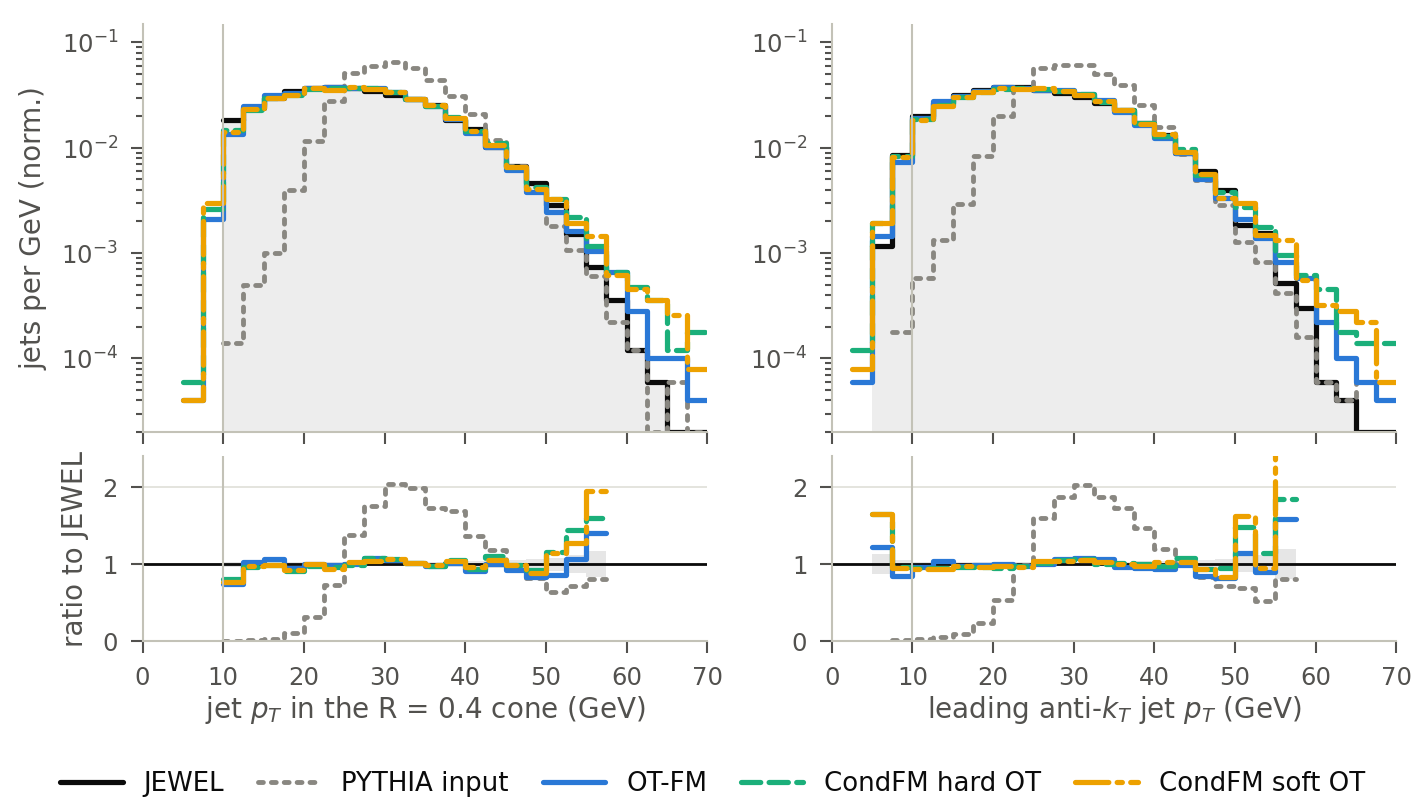
\includegraphics[width=\textwidth]{deck_pt.png}
\column{0.62\textwidth}
\scriptsize
\begin{itemize}\setlength\itemsep{0.2em}
\item \textbf{Shapes} as close to JEWEL as \ot{}'s, also at fixed $p_T$ and for re-found jets
\item \textbf{$p_T$ and mass} 2-3$\times$ \ot{}'s distance (too many jets above 50 GeV): 2.7-2.9 sd
  (\hda{}), mass 3.4 sd (\sfa{}). A second sampler seed moves every distance by $\le$ 0.011
\item \textbf{Single jets sharp:} occupancy, leading tower, core and soft energy as JEWEL's; 5\% of
  samples in JEWEL's 5\% tails; no flag
\item \textbf{The input sets little of the output $p_T$:} $r = 0.19$ (\ot{} 0.94); median output 23 GeV
  for 20-25 GeV inputs, 30 GeV for 50-70 GeV inputs
\end{itemize}
\end{columns}
\end{frame}

% ---------------------------------------------------------------- S3
\begin{frame}{S3. Eight samples per jet: how much they differ, and what they follow}
\begin{columns}[T]
\column{0.58\textwidth}
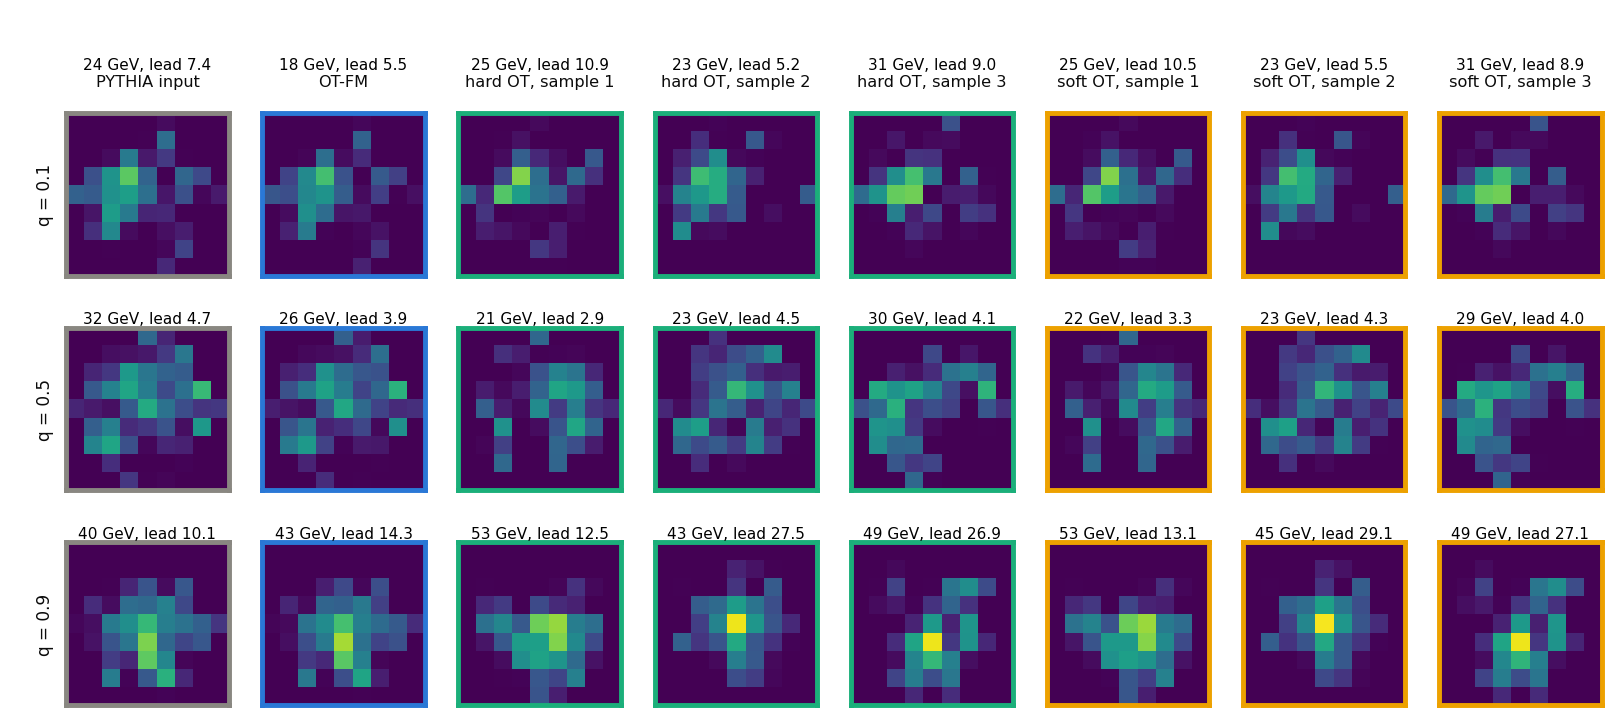
\includegraphics[width=\textwidth]{cf_samples_slide.png}

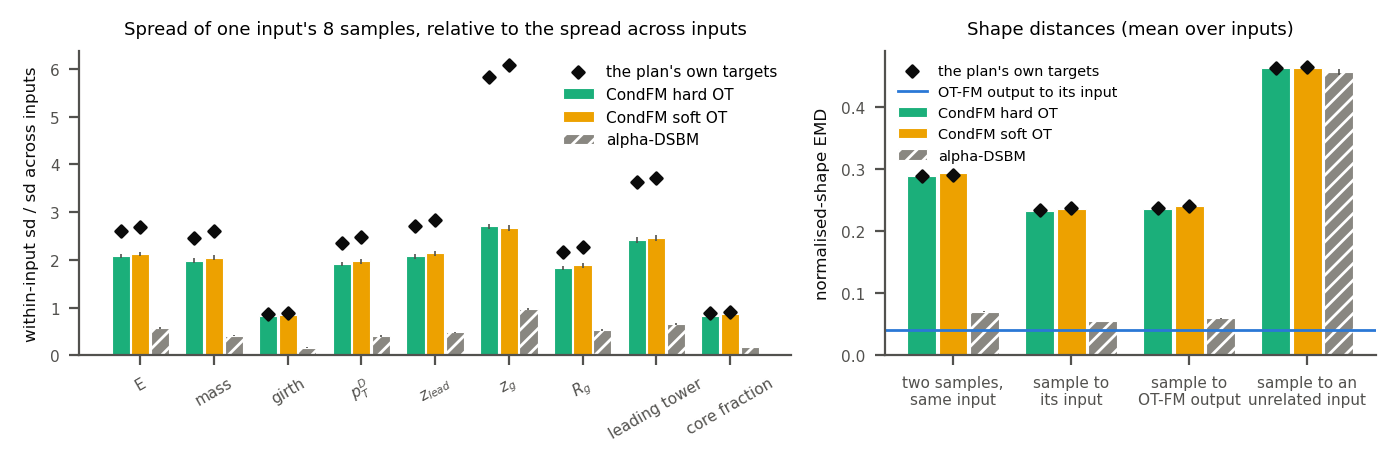
\includegraphics[width=\textwidth]{cf_spread.png}
\column{0.4\textwidth}
\scriptsize
\begin{itemize}\setlength\itemsep{0.15em}
\item \textbf{Large, real diversity:} two samples of one jet differ by 13 GeV rms in $p_T$ and 0.29 in
  shape EMD, more than a sample differs from its input (0.23; unrelated jets 0.47; \ot{}'s change 0.04;
  solver 0.005 GeV)
\item \textbf{Not only energy:} within one input $p_T^D$, $z_\mathrm{lead}$, $z_g$, $R_g$ spread as much
  as over all JEWEL jets, girth and core 65\% as much; coherently ($p_T$ with lead tower $r$ 0.78)
\item \textbf{The pairing's spread ($\blacklozenge$):} the targets each plan assigns to the same inputs
  spread and correlate with them as the samples do (table)
\item \textbf{Swap $c$ at fixed $\epsilon$:} the output follows the new jet's shape (93\% closer to it
  than to the old input); the noise adds a shared $p_T$ and width shift ($r$ 0.39, 0.52)
\item \textbf{\hda{} = \sfa{}:} same input and noise: 0.012 in shape EMD, 0.8 GeV apart
\end{itemize}
\vspace{0.1em}
\scriptsize
\setlength{\tabcolsep}{3pt}
\begin{tabular}{lrrrrr}
\toprule
$r$(sample, input) & $p_T$ & mass & girth & $z_\mathrm{lead}$ & core \\
\midrule
\keyot OT-FM & 0.94 & 0.92 & 0.99 & 0.96 & 0.99 \\
\keyhd hard OT & 0.17 & 0.25 & 0.73 & 0.24 & 0.72 \\
\quad its pairs & 0.16 & 0.25 & 0.72 & 0.24 & 0.71 \\
\keysf soft OT & 0.16 & 0.24 & 0.72 & 0.22 & 0.71 \\
\quad its pairs & 0.15 & 0.23 & 0.71 & 0.23 & 0.70 \\
\bottomrule
\end{tabular}

\end{columns}
\end{frame}

% ---------------------------------------------------------------- S4
\begin{frame}{S4. Reading and cost}
\begin{columns}[T]
\column{0.5\textwidth}
\scriptsize
\textbf{Pre-registered reading}

\vspace{0.15em}
\scriptsize
\setlength{\tabcolsep}{3pt}
\begin{tabular}{lll}
\toprule
 & \keyhd hard OT & \keysf soft OT \\
\midrule
toward JEWEL ($\geq$ 4 of 7, both joints) & \textbf{yes} (6 of 7) & \textbf{yes} (6 of 7) \\
none 3 sd worse than OT-FM & \textbf{yes} & no (mass) \\
input dependence beyond random & \textbf{yes} & \textbf{yes} \\
sharp samples (tails $\leq$ 10\%) & \textbf{yes} (5\%, 5\%) & \textbf{yes} (5\%, 6\%) \\
solver resolved & \textbf{yes} & \textbf{yes} \\
diversity above numerical error & \textbf{yes} & \textbf{yes} \\
follows the condition (swap) & \textbf{yes} (66\%) & \textbf{yes} (64\%) \\
\textbf{useful (all of the above)} & \textbf{yes} & no \\
\bottomrule
\end{tabular}


\vspace{0.5em}
\textbf{Cost} {\color{ink2}(one A6000 each; training time; latency at batch 2000)}

\vspace{0.15em}
\scriptsize
\setlength{\tabcolsep}{3pt}
\begin{tabular}{lrrrrrr}
\toprule
 & GPU h & updates & per s & OT & calls & ms/jet \\
\midrule
\keyot OT-FM & 2.00 & 123k & 17.0 & 10\% & 128 & 6.58 \\
\keyhd hard OT & 2.00 & 122k & 17.0 & 10\% & 128 & 6.60 \\
\keysf soft OT & 2.00 & 121k & 16.9 & 11\% & 128 & 6.67 \\
$\alpha$-DSBM & 2.00 & 35k & -- & -- & 30 & 1.55 \\
CycleGAN 2 h & 2.06 & 20k & -- & -- & 1 & 0.05 \\
\bottomrule
\end{tabular}

\column{0.48\textwidth}
\scriptsize
\begin{itemize}\setlength\itemsep{0.35em}
\item \textbf{By the letter} \hda{} meets every item; \sfa{} misses one (mass 3.4 sd behind \ot{}).
\item \textbf{What the samples are:} sharp JEWEL-like jets that share part of the input's width and
  core and little of its $p_T$. The model learned its pairing's conditional distribution faithfully;
  a minibatch-OT pair keeps $r(p_T) = 0.17$. \ot{}'s tight per-jet relation ($r = 0.94$) comes from the
  deterministic flow, not from the pairs.
\item \textbf{More spread is not better here:} the spread is the pairing's, not a medium fluctuation;
  the entropic plan adds nothing measurable to the variety of the hard plan's partners.
\item \textbf{Variability:} all spreads are sampling variability of one trained model per arm; a second
  sampler seed moves the benchmark by about one bootstrap sd; training-seed variability is not measured.
\item \textbf{Not shown:} a physical medium response, a calibrated uncertainty, a per-jet truth. Keeping
  the input $p_T$ would need a pairing that keeps it: a modelling choice unpaired data cannot make.
\end{itemize}
\end{columns}
\end{frame}

\end{document}
